\subsubsection{Running a geodynamic model}
\label{sec:cookbooks-running-a-model}
\textit{This section was contributed by Juliane Dannberg.}

The input file for this model can be found at \url{cookbooks/convection-box-particles/convection-box-particles.prm}.

This model is a modification of the Convection in a 2d box cookbook described in section \ref{sec:cookbooks-simple-box}. 
It is changed to a lower resolution, uses physical units, and outputs particles, which can be used to visualize the flow 
of the material. 
This makes it a good setup to run as a very first simple geodynamic model to test if \aspect{} is running on everyone's
computer, and to demonstrate how to visualize models results. 

\begin{figure}[h]
\phantom.
\hfill
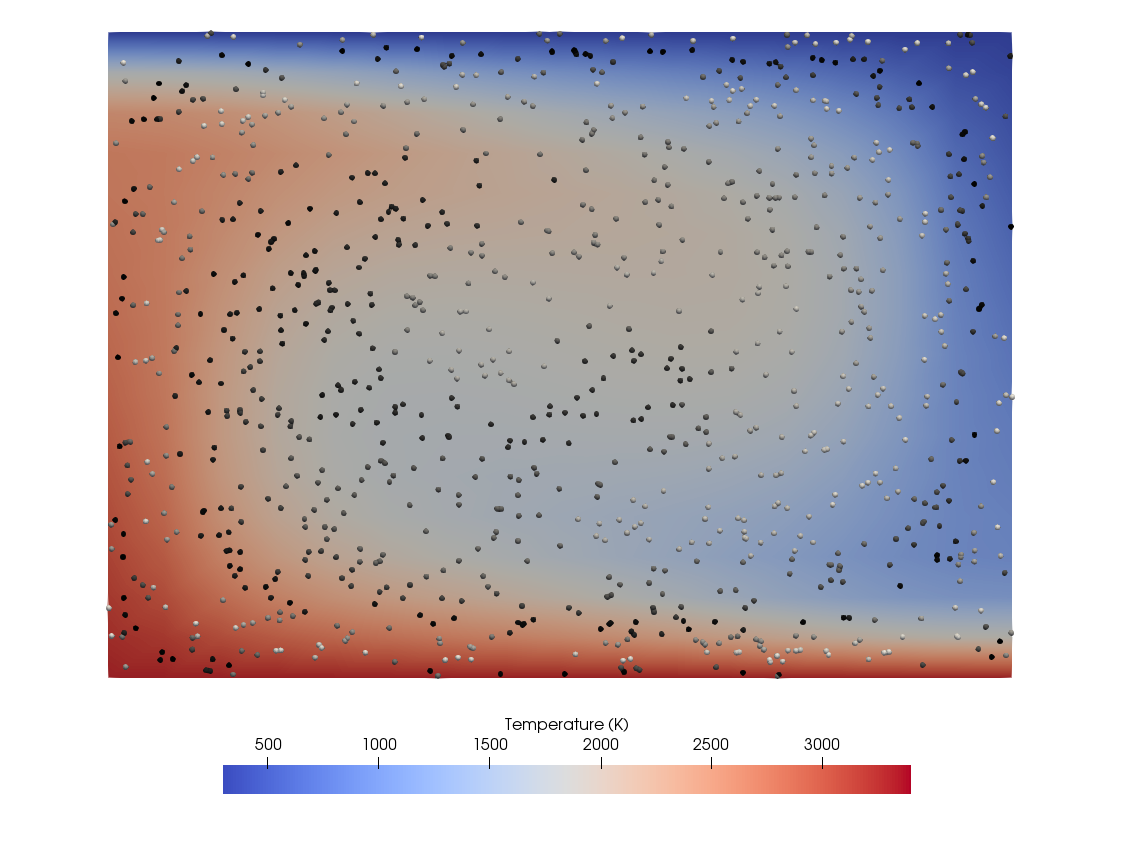
\includegraphics[width=0.4\textwidth]{convection-box.png}
\hfill
\phantom.
\caption{\it Setup of the tutorial model. Background colors show temperature, gray spheres illustrate particle positions.}
\label{fig:convection-box-iterations}
\end{figure}

Slides that demonstrate how to run the model from inside a virtual machine, and how to use ParaView to look at the model
output can be found \href{https://www.dropbox.com/s/dmlcf4tx62ts6d1/02_geophysics_tutorial_01_08.pdf?dl=0}{here}. 
The model can also be used to show how the thermal conductivity (or other physical parameters that change the Rayleigh
number) control the vigor of convection. An example for this is given in \href{https://www.dropbox.com/s/nqkxe54poe1op7d/03_geophysics_lecture_01_10.pdf?dl=0}{this presentation (last slide)}.



